% Mock Viva Presentation — AI-Assisted Epilepsy Detection using EEG Signals
% Compile: xelatex mock_viva_slides.tex
\documentclass[aspectratio=169,12pt]{beamer}

\usetheme{Madrid}
\usecolortheme{default}
\definecolor{qmblue}{RGB}{0,74,127}
\setbeamercolor{structure}{fg=qmblue}
\setbeamercolor{title}{fg=white,bg=qmblue}
\setbeamercolor{frametitle}{fg=white,bg=qmblue}
\setbeamercolor{block title}{fg=white,bg=qmblue}
\setbeamertemplate{navigation symbols}{}
\setbeamertemplate{footline}{%
  \leavevmode\hbox{%
    \begin{beamercolorbox}[wd=.333\paperwidth,ht=2.5ex,dp=1ex,center]{author in head/foot}%
      \usebeamerfont{author in head/foot}\insertshortauthor
    \end{beamercolorbox}%
    \begin{beamercolorbox}[wd=.334\paperwidth,ht=2.5ex,dp=1ex,center]{title in head/foot}%
      \usebeamerfont{title in head/foot}\insertshorttitle
    \end{beamercolorbox}%
    \begin{beamercolorbox}[wd=.333\paperwidth,ht=2.5ex,dp=1ex,right]{date in head/foot}%
      \usebeamerfont{date in head/foot}%
      \insertframenumber{} / \inserttotalframenumber\hspace*{2ex}
    \end{beamercolorbox}%
  }%
}

\usepackage{fontspec}
\usepackage{graphicx}
\usepackage{booktabs}
\usepackage{multirow}
\usepackage{array}
\usepackage{xcolor}
\usepackage{tikz}
\usepackage{eso-pic}

\graphicspath{{../BBC6521_Final_Report_LaTeX_Template_25_26/figures/}}

\pgfdeclareimage[height=0.7cm]{qmlogo}{logo_QM_white.png}

\AddToShipoutPictureFG{%
  \ifnum\value{page}>1
    \begin{tikzpicture}[remember picture,overlay]
      \node[anchor=north east,xshift=-8pt,yshift=-3pt] at (current page.north east) {\pgfuseimage{qmlogo}};
    \end{tikzpicture}%
  \fi
}

\title[AI-Assisted Epilepsy Detection]{AI-Assisted Epilepsy Detection\\using EEG Signals}
\author[Zhong Ziwen]{Zhong Ziwen\\{\small BUPT No. 2022213356\quad QMUL No. 221168280}}
\institute[BUPT-QMUL]{Internet of Things Engineering\\BUPT-QMUL Joint Programme}
\date{April 2026}

\begin{document}

%=== Slide 1: Title ===
\begin{frame}
\titlepage
\end{frame}

%=== Slide 2: Outline ===
\begin{frame}{Outline}
\tableofcontents[hideallsubsections]
\end{frame}

%---------------------------------------------------------------
\section{Background and Motivation}
%---------------------------------------------------------------

%=== Slide 3: Problem and Motivation ===
\begin{frame}{Problem and Motivation}
\begin{itemize}\itemsep4pt
    \item Epilepsy affects \textbf{50 million} people worldwide; \textbf{30\%} have drug-resistant epilepsy requiring long-term EEG monitoring
    \item Clinical diagnosis relies on \textbf{visual inspection} of EEG by neurologists
    \begin{itemize}\itemsep2pt\small
        \item Hours of multi-channel recordings per patient --- extremely time-consuming
        \item High \textbf{inter-rater variability} --- subjective interpretation leads to inconsistent diagnoses
        \item Shortage of trained neurologists, especially in developing regions
    \end{itemize}
    \item Automated EEG analysis can provide \textbf{objective}, \textbf{consistent}, and \textbf{scalable} diagnostic support
    \item Evolution of automated methods:
    \begin{itemize}\small
        \item Traditional ML: hand-crafted features (wavelet, entropy) + SVM / Random Forest
        \item Deep learning: CNN (spatial) $\rightarrow$ RNN/LSTM (temporal) $\rightarrow$ \textbf{hybrid architectures}
        \item Hybrid models combine strengths of multiple components, but lack rigorous evaluation
    \end{itemize}
\end{itemize}
\end{frame}

%=== Slide 4: Research Gaps and Objectives ===
\begin{frame}[shrink=3]{Research Gaps and Objectives}
\begin{columns}[T]
\begin{column}{0.48\textwidth}
\textbf{Three critical gaps in existing literature:}
\begin{enumerate}\itemsep4pt\small
    \item \textcolor{red}{\textbf{Data leakage}} --- Most studies (e.g., Thara 2019) split at \textit{segment level}; overlapping sliding windows from the same recording appear in both train and test $\rightarrow$ artificially inflated accuracy
    \item \textbf{Lack of ablation studies} --- Hybrid models are proposed as a whole, rarely decomposed to verify each component's contribution (Shoeibi 2021)
    \item \textbf{Limited multi-class evaluation} --- Binary (normal vs seizure) is dominant; clinically important \textit{interictal} states are often ignored
\end{enumerate}
\end{column}
\begin{column}{0.48\textwidth}
\textbf{Project objectives:}
\begin{enumerate}\itemsep4pt\small
    \item Implement \textbf{recording-level} 10-Fold CV to eliminate data leakage entirely
    \item Design a lightweight hybrid \textbf{CNN + Bi-LSTM + Self-Attention} architecture ($\sim$500K params)
    \item Conduct systematic \textbf{ablation}: 3 baselines (Pure CNN, Pure BiLSTM, SVM+WPD)
    \item Evaluate across \textbf{3 tasks} of increasing difficulty: binary, three-class, five-class
    \item Visualise attention weights to enhance \textbf{clinical interpretability}
\end{enumerate}
\end{column}
\end{columns}
\end{frame}

%---------------------------------------------------------------
\section{Dataset and Preprocessing}
%---------------------------------------------------------------

%=== Slide 5: Bonn EEG Dataset ===
\begin{frame}[shrink=5]{Dataset --- University of Bonn EEG}
\begin{columns}[T]
\begin{column}{0.55\textwidth}
\small
\begin{itemize}\itemsep2pt
    \item \textbf{5 subsets}, 100 single-channel recordings each (500 total)
    \item 173.61\,Hz sampling, 23.6\,s/recording, 4097 points
    \item Bandpass filtered 0.53--40\,Hz during acquisition
\end{itemize}
\vspace{0.15cm}
\scriptsize
\begin{tabular}{llll}
\toprule
\textbf{Set} & \textbf{Subject} & \textbf{State} & \textbf{EEG Type}\\
\midrule
Z & Healthy & Eyes open & Surface\\
O & Healthy & Eyes closed & Surface\\
N & Epileptic & Interictal, contralateral & Intracranial\\
F & Epileptic & Interictal, epileptogenic & Intracranial\\
S & Epileptic & \textbf{Seizure (ictal)} & Intracranial\\
\bottomrule
\end{tabular}
\vspace{0.15cm}

\scriptsize
\begin{tabular}{lll}
\toprule
\textbf{Task} & \textbf{Classes} & \textbf{Rec.}\\
\midrule
Binary & Normal (Z+O) vs Seizure (S) & 300\\
Three-class & Normal vs Interictal vs Seizure & 500\\
Five-class & Z / O / N / F / S & 500\\
\bottomrule
\end{tabular}
\end{column}
\begin{column}{0.42\textwidth}
\centering
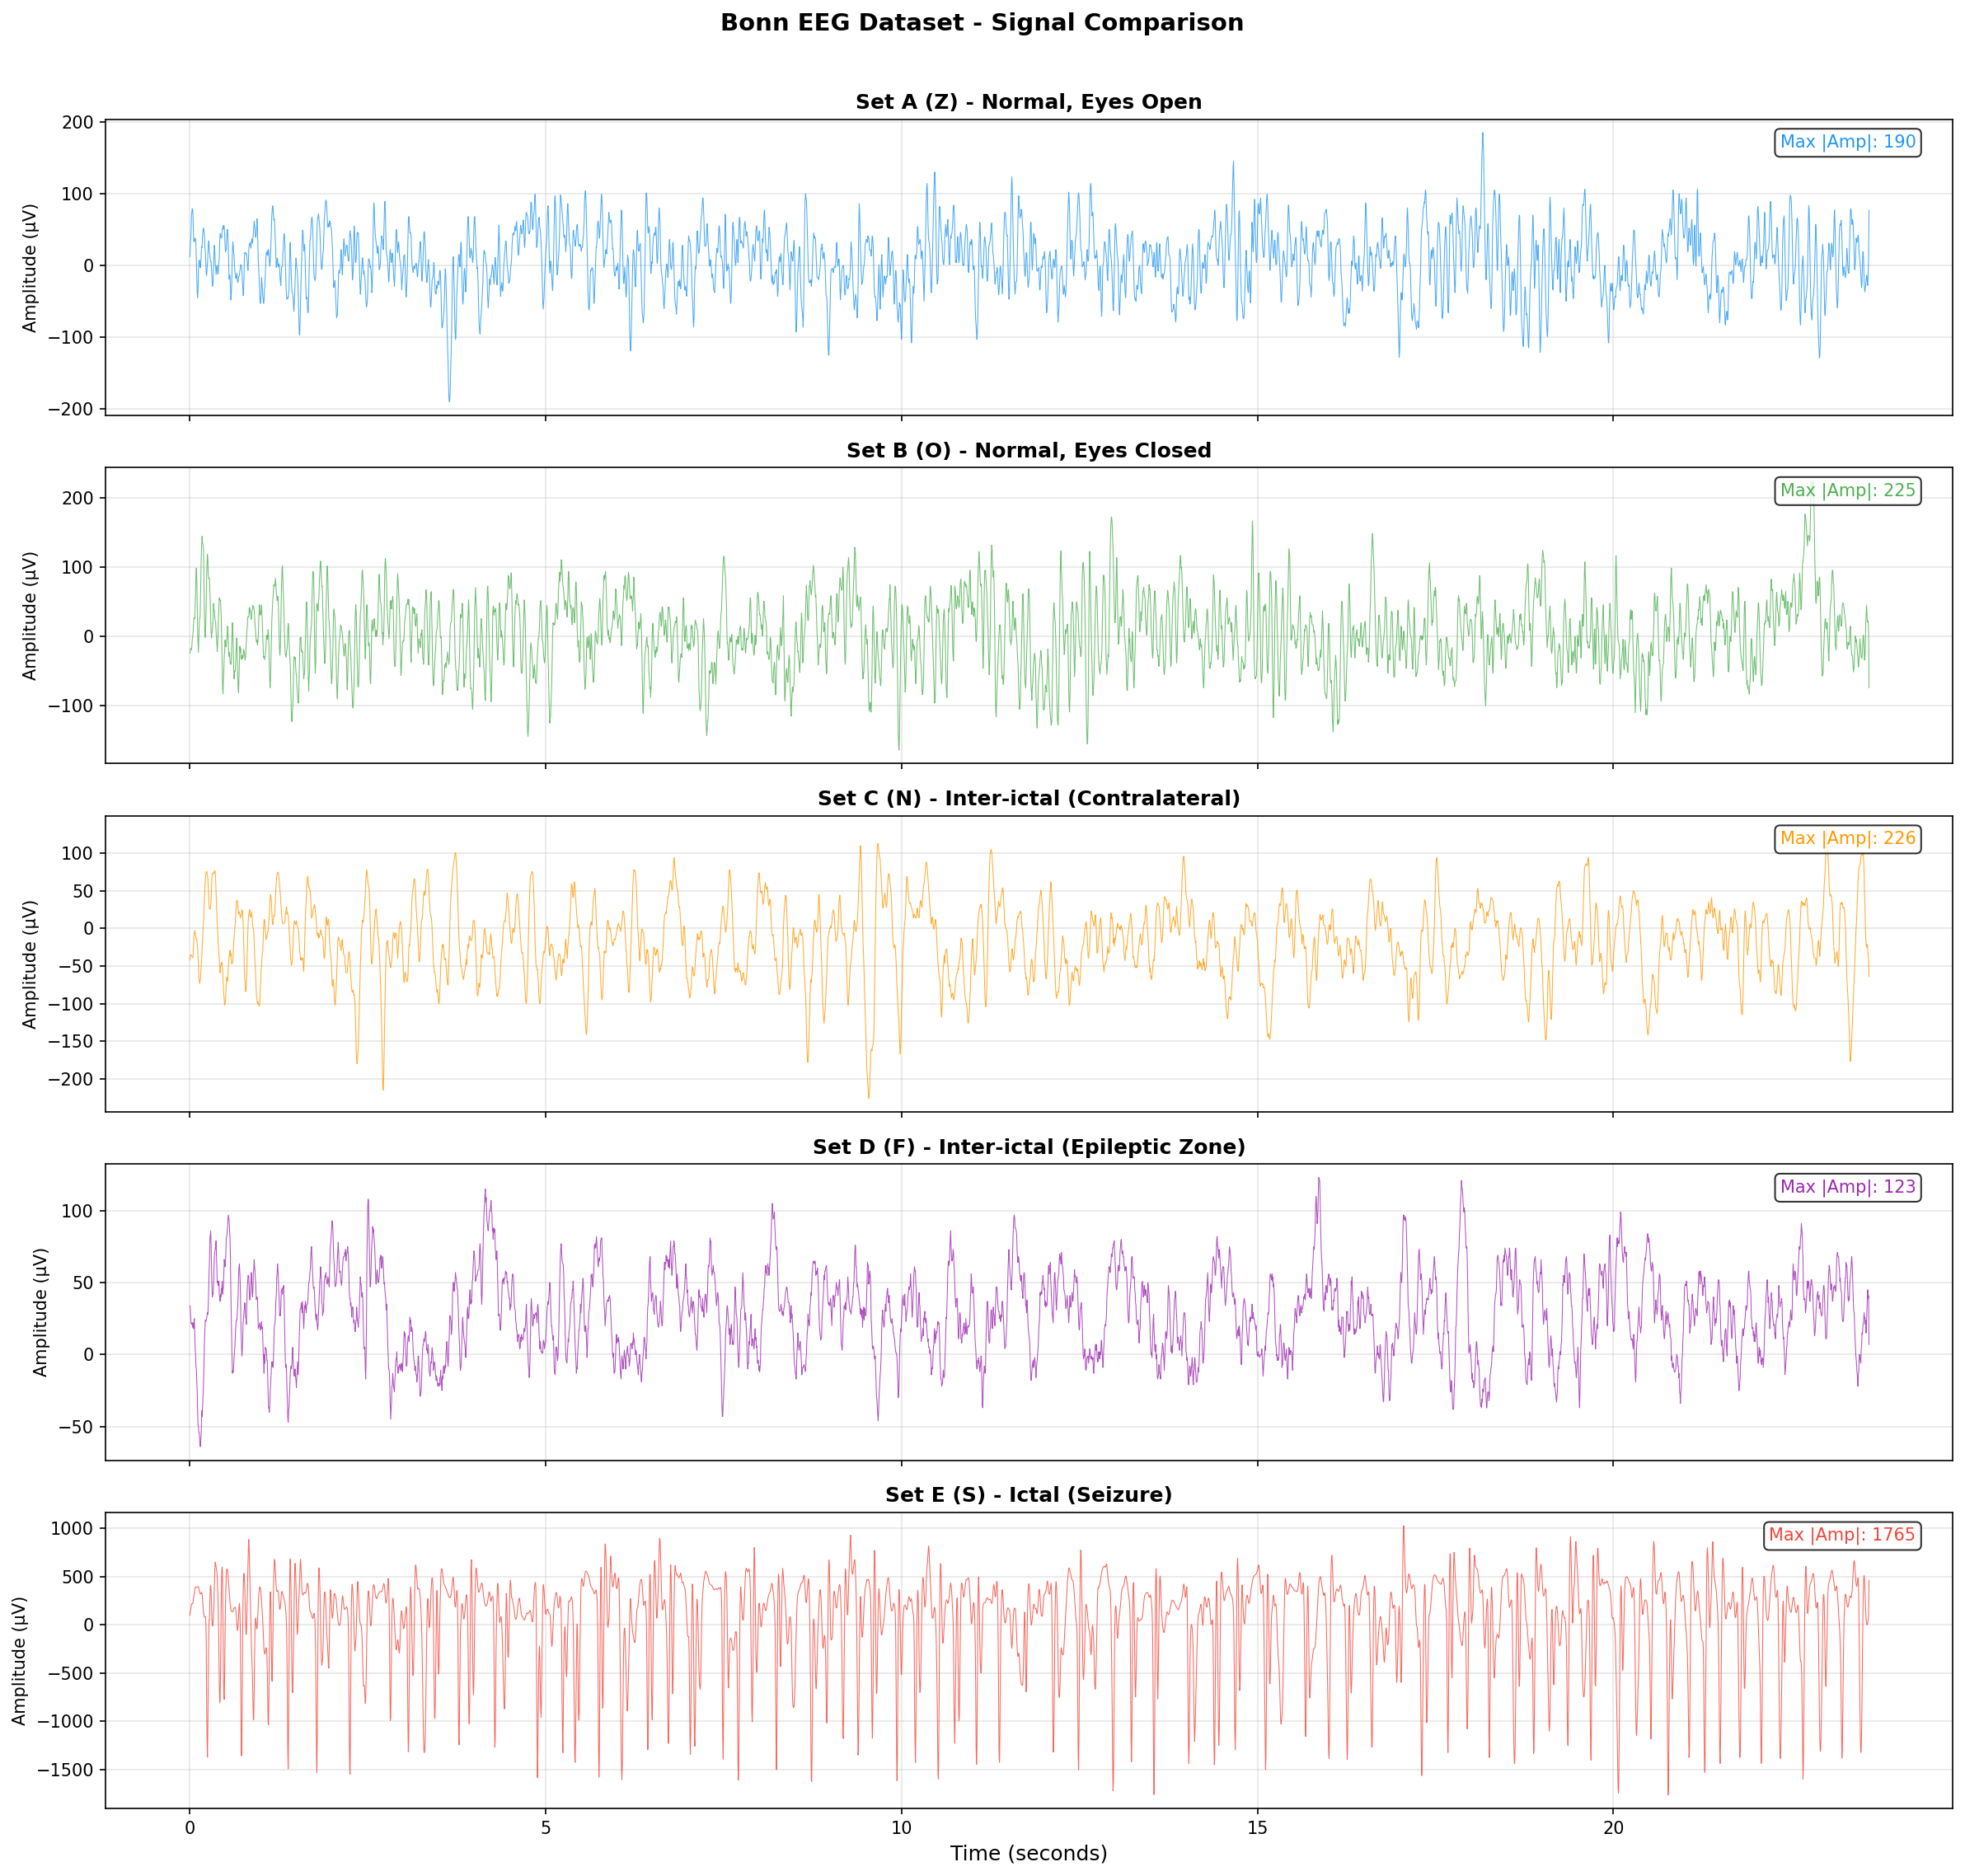
\includegraphics[width=\linewidth]{signal_comparison.png}\\
{\scriptsize EEG waveform comparison across five subsets: Normal (Z, O) shows regular low-amplitude activity; Seizure (S) shows high-amplitude rhythmic discharges}
\end{column}
\end{columns}
\end{frame}

%=== Slide 6: Data Leakage Problem ===
\begin{frame}{Data Leakage: Problem and Solution}
\begin{block}{The Problem --- Commonly Overlooked in Literature}
\small
Many studies (e.g., Thara 2019) split EEG \textit{segments} randomly. With 50\% overlapping windows, adjacent segments from the \textbf{same recording} share up to half their data points $\rightarrow$ model memorises patterns $\rightarrow$ \textbf{artificially inflated accuracy}.
\end{block}

\vspace{0.1cm}
\begin{block}{Our Solution --- Recording-Level 10-Fold Cross-Validation}
\small
\begin{itemize}\itemsep0pt
    \item Split at \textbf{recording level}: 500 recordings assigned to folds \textbf{before} any windowing
    \item Each fold: 450 train / 50 validate --- \textbf{zero overlap} between sets
    \item Sliding windows (1024 pts, 50\% overlap) generated \textbf{independently within each set}
    \item StandardScaler \textbf{fit on training windows only}, then applied to validation
\end{itemize}
\end{block}

\vspace{0.05cm}
\centering
{\scriptsize\textit{Discovered during development when initial accuracy seemed suspiciously high.} After fix, results remain strong and consistent with peer-reviewed benchmarks.}
\end{frame}

%=== Slide 7: Preprocessing Pipeline ===
\begin{frame}{Preprocessing Pipeline}
\begin{columns}[c]
\begin{column}{0.56\textwidth}
\centering
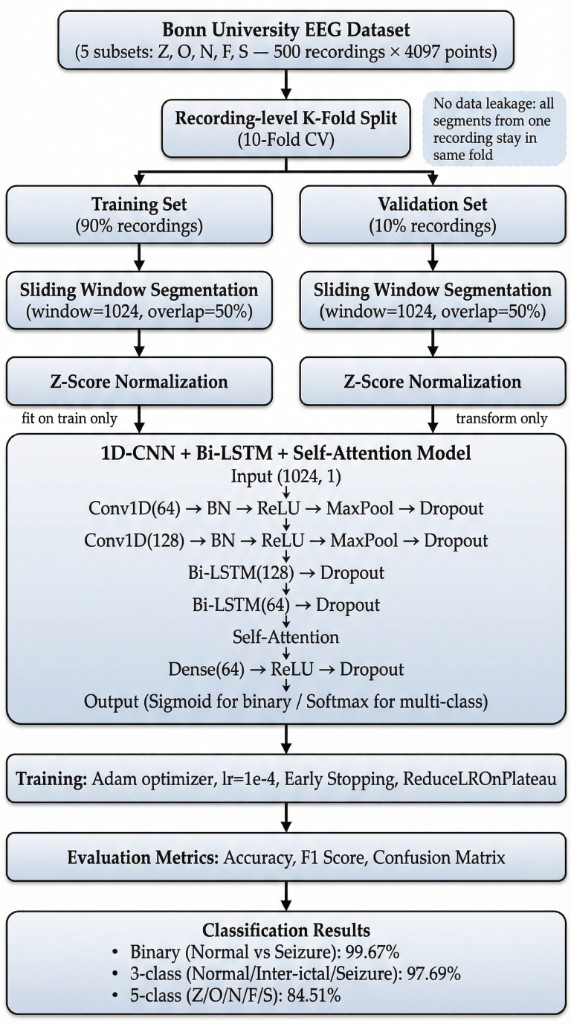
\includegraphics[width=\linewidth,height=0.8\textheight,keepaspectratio]{preprocessing_pipeline.png}
\end{column}
\begin{column}{0.42\textwidth}
\small
\textbf{1. Recording-level Split}\\[2pt]
{\scriptsize 500 recordings $\rightarrow$ 10 folds.\\All windows from one recording stay in the same fold.}

\vspace{0.25cm}
\textbf{2. Sliding Window}\\[2pt]
{\scriptsize 1024 points ($\sim$5.9\,s), 50\% overlap.\\Applied independently per fold.}

\vspace{0.25cm}
\textbf{3. Z-Score Normalisation}\\[2pt]
{\scriptsize Global mean/std computed on \textbf{training set only}; applied to validation set.}

\vspace{0.25cm}
\textbf{4. No Extra Filtering}\\[2pt]
{\scriptsize Bonn dataset already bandpass filtered at 0.53--40\,Hz during acquisition.}
\end{column}
\end{columns}
\end{frame}

%---------------------------------------------------------------
\section{Proposed Method}
%---------------------------------------------------------------

%=== Slide 8: Hybrid Model Architecture ===
\begin{frame}{Proposed Hybrid Model Architecture}
\centering
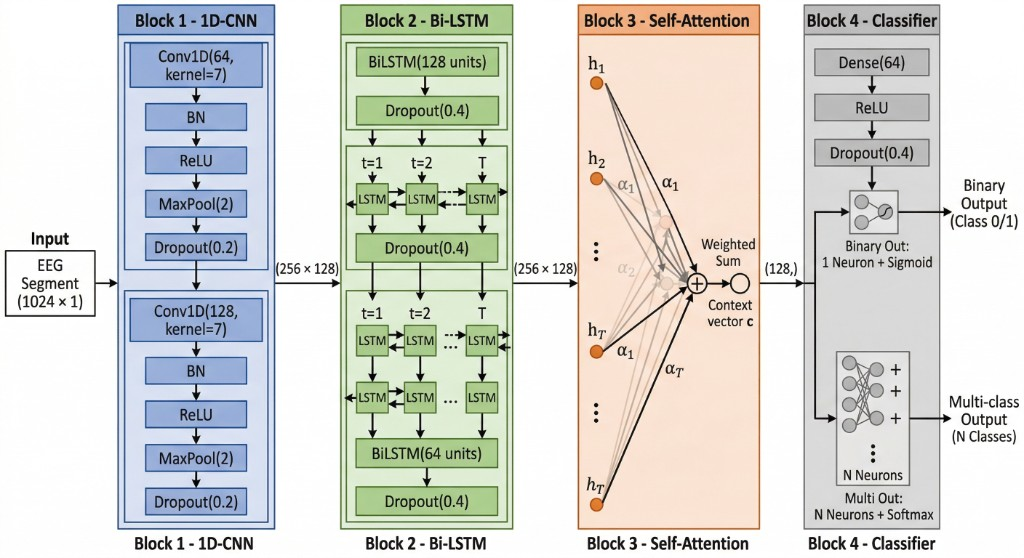
\includegraphics[width=0.75\linewidth,height=0.55\textheight,keepaspectratio]{model_architecture.png}

\vspace{0.15cm}
\begin{columns}[T]
\begin{column}{0.32\textwidth}
\centering
\textbf{1D-CNN}\\
{\scriptsize 2 Conv layers (64, 128)\\Local morphological features\\(spike shape, sharp waves)}
\end{column}
\begin{column}{0.32\textwidth}
\centering
\textbf{Bi-LSTM}\\
{\scriptsize 2 layers (128, 64 units)\\Bidirectional temporal\\dependency modelling}
\end{column}
\begin{column}{0.32\textwidth}
\centering
\textbf{Self-Attention}\\
{\scriptsize $\text{softmax}(QK^\top\!/\sqrt{d_k})\,V$\\Focus on clinically\\relevant time steps}
\end{column}
\end{columns}
\vspace{0.1cm}
\centering
{\scriptsize Output: Dense(64) $\rightarrow$ ReLU $\rightarrow$ Dropout $\rightarrow$ Softmax\quad|\quad Total: $\sim$\textbf{500K} parameters}
\end{frame}

%=== Slide 9: Ablation Design ===
\begin{frame}[shrink=3]{Ablation Study Design}
\begin{table}
\centering
\small
\begin{tabular}{lcccl}
\toprule
\textbf{Model} & \textbf{CNN} & \textbf{BiLSTM} & \textbf{Attention} & \textbf{Purpose}\\
\midrule
\textbf{Hybrid (ours)} & \checkmark & \checkmark & \checkmark & Full proposed model\\
Pure CNN & \checkmark & & & Spatial features only\\
Pure BiLSTM+Attn & & \checkmark & \checkmark & Temporal features only\\
SVM + WPD & \multicolumn{3}{c}{(traditional ML)} & Non-DL baseline\\
\bottomrule
\end{tabular}
\end{table}

\vspace{0.15cm}
\begin{itemize}\small\itemsep2pt
    \item \textbf{Controlled comparison}: all DL models share identical preprocessing, data splits, and 10-Fold CV protocol --- only the architecture varies
    \item \textbf{SVM baseline}: Wavelet Packet Decomposition (3-level, `db4') extracts energy and Shannon entropy features per subband; RBF kernel SVM classifier
    \item \textbf{Ablation logic}: removing CNN isolates temporal modelling (BiLSTM); removing BiLSTM+Attention isolates spatial features (CNN); SVM tests traditional ML upper bound
    \item \textbf{Training}: Adam optimiser, lr=$10^{-4}$, early stopping (patience=10), ReduceLROnPlateau; trained on RTX 3070 Ti, 50 epochs per fold
\end{itemize}
\end{frame}

%---------------------------------------------------------------
\section{Results and Discussion}
%---------------------------------------------------------------

%=== Slide 10: Binary and Three-class Results ===
\begin{frame}[shrink=3]{Results --- Binary and Three-class Classification}
\begin{columns}[T]
\begin{column}{0.48\textwidth}
\centering
\textbf{Binary: Normal (Z+O) vs Seizure (S)}\\[0.15cm]
\small
\begin{tabular}{lcc}
\toprule
\textbf{Model} & \textbf{Acc (\%)} & \textbf{F1}\\
\midrule
SVM+WPD & 99.67\scriptsize{$\pm$1.00} & 99.66\\
Pure CNN & 98.86\scriptsize{$\pm$1.91} & 98.84\\
BiLSTM+Attn & 99.48\scriptsize{$\pm$1.29} & 99.47\\
\textbf{Hybrid} & \textbf{99.67}\scriptsize{$\pm$0.85} & \textbf{99.66}\\
\bottomrule
\end{tabular}
\vspace{0.15cm}

{\scriptsize Binary task is inherently simple due to\\distinct morphological differences between\\normal and seizure signals. All models $>$98\%.}
\end{column}
\begin{column}{0.48\textwidth}
\centering
\textbf{Three-class: Normal / Interictal / Seizure}\\[0.15cm]
\small
\begin{tabular}{lcc}
\toprule
\textbf{Model} & \textbf{Acc (\%)} & \textbf{F1}\\
\midrule
SVM+WPD & 94.20\scriptsize{$\pm$2.44} & 94.19\\
Pure CNN & 97.14\scriptsize{$\pm$1.84} & 97.11\\
BiLSTM+Attn & 92.80\scriptsize{$\pm$5.99} & 92.74\\
\textbf{Hybrid} & \textbf{97.69}\scriptsize{$\pm$2.17} & \textbf{97.68}\\
\bottomrule
\end{tabular}
\vspace{0.15cm}

{\scriptsize Introducing interictal class increases difficulty.\\BiLSTM alone drops to 92.80\% with high variance\\($\pm$5.99), while Hybrid remains stable at 97.69\%.}
\end{column}
\end{columns}
\end{frame}

%=== Slide 11: Five-class Results ===
\begin{frame}[shrink=2]{Results --- Five-class Classification}
\begin{columns}[T]
\begin{column}{0.48\textwidth}
\centering
\small
\begin{tabular}{lcc}
\toprule
\textbf{Model} & \textbf{Acc (\%)} & \textbf{F1}\\
\midrule
SVM+WPD & 78.80\scriptsize{$\pm$5.31} & 78.39\\
Pure CNN & 78.86\scriptsize{$\pm$3.77} & 75.95\\
BiLSTM+Attn & 73.09\scriptsize{$\pm$8.37} & 71.92\\
\textbf{Hybrid} & \textbf{84.51}\scriptsize{$\pm$3.62} & \textbf{84.28}\\
\bottomrule
\end{tabular}

\vspace{0.2cm}
\begin{itemize}\small\itemsep2pt
    \item Hybrid leads CNN by \textbf{+5.65\%}
    \item Hybrid leads BiLSTM by \textbf{+11.42\%}
    \item CNN captures local shape but misses long-range context; BiLSTM lacks spatial precision
    \item \textbf{Synergy} of all three components is most evident in this hardest task
\end{itemize}
\end{column}
\begin{column}{0.48\textwidth}
\centering
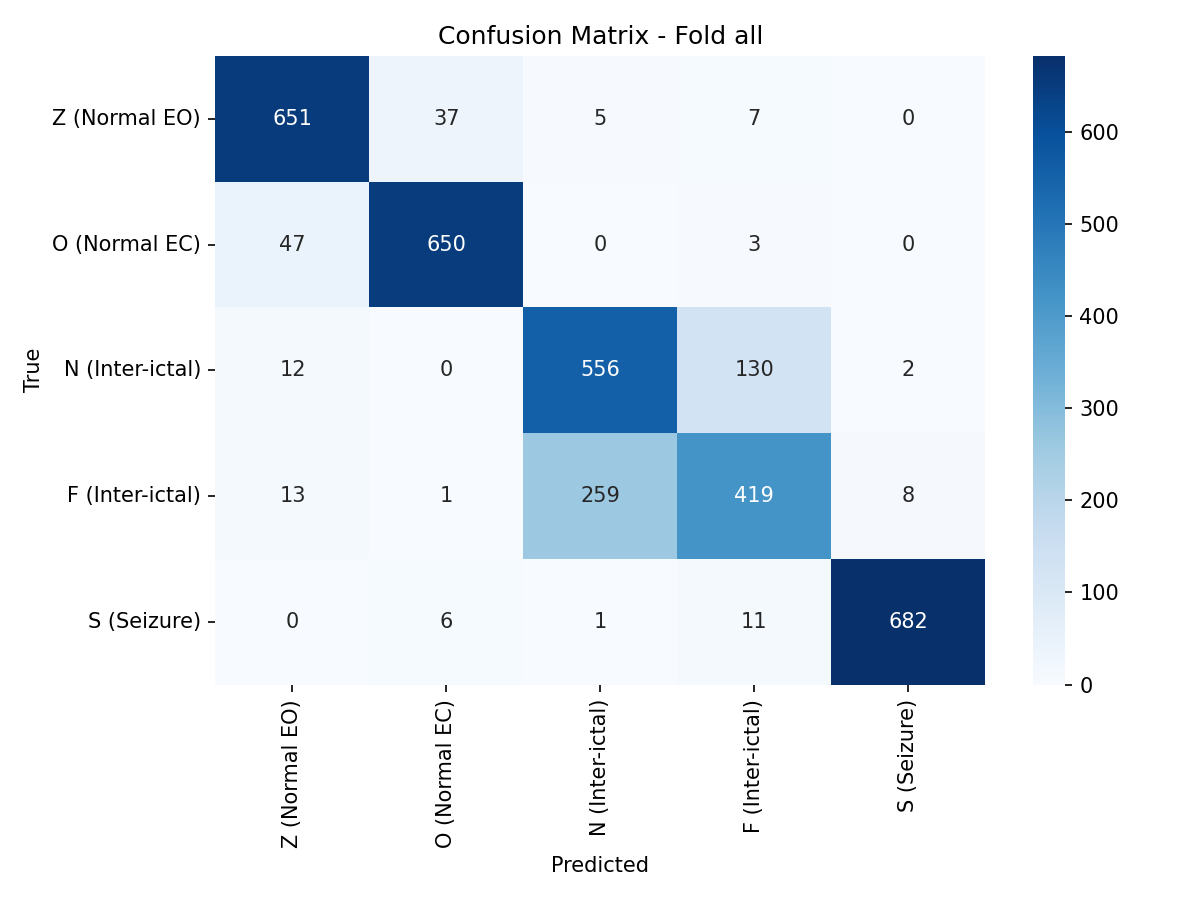
\includegraphics[width=\linewidth]{cm_five_hybrid.png}\\
{\scriptsize Five-class confusion matrix (Hybrid model).\\Main errors: N$\leftrightarrow$F mutual confusion --- both are interictal recordings with similar morphology.\\Z and S classes achieve near-perfect classification.}
\end{column}
\end{columns}
\end{frame}

%=== Slide 12: Attention Visualisation ===
\begin{frame}{Attention Weight Visualisation}
\begin{columns}[c]
\begin{column}{0.52\textwidth}
\centering
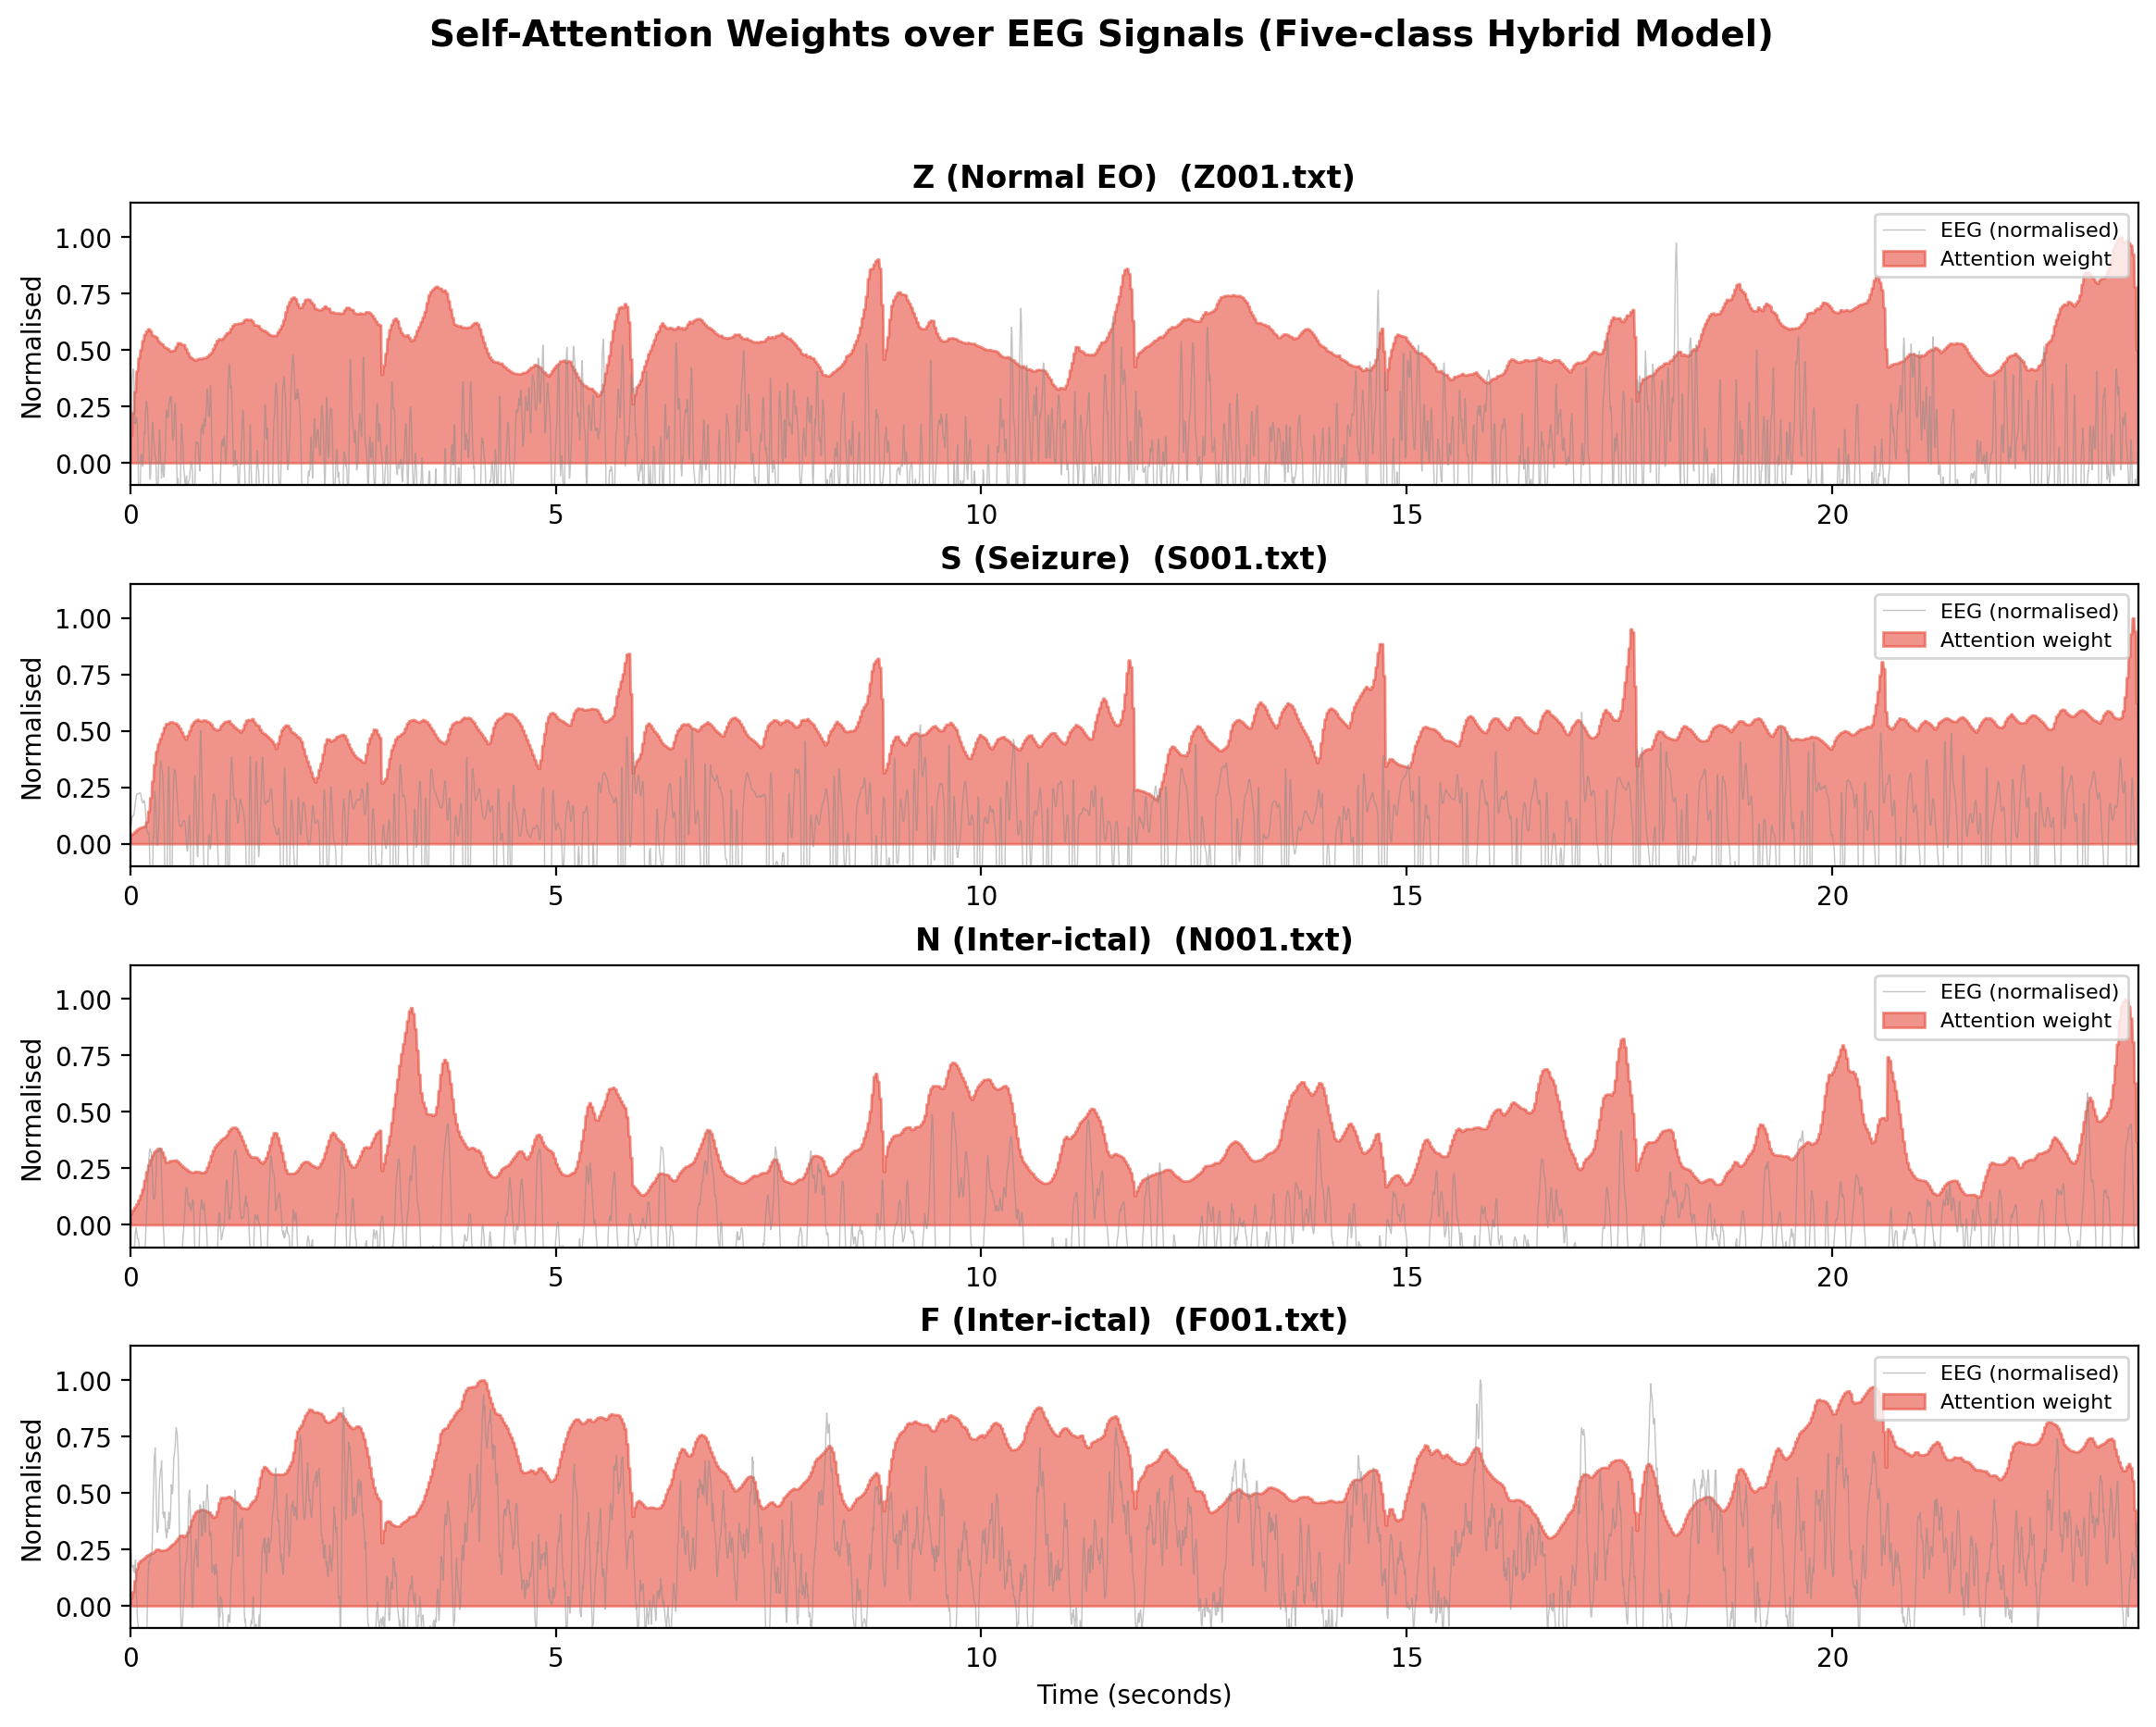
\includegraphics[width=\linewidth,height=0.72\textheight,keepaspectratio]{attention_heatmap.png}
\end{column}
\begin{column}{0.46\textwidth}
\small
\textbf{Class-specific attention patterns:}
\begin{itemize}\itemsep2pt\small
    \item \textbf{Seizure (S)}: high weights on \textit{sharp waves} and \textit{high-frequency bursts} --- hallmark of ictal activity
    \item \textbf{Normal (Z, O)}: weights distributed \textit{uniformly} --- no dominant abnormal region
    \item \textbf{Interictal (N, F)}: moderate peaks on subtle \textit{spike-and-wave} complexes
\end{itemize}

\vspace{0.1cm}
{\scriptsize \textbf{Clinical significance}: Attention aligns with features neurologists look for during visual EEG review. This ``white-box'' property supports clinical trust in AI-assisted diagnosis.}
\end{column}
\end{columns}
\end{frame}

%=== Slide 13: Statistical Testing and Literature Comparison ===
\begin{frame}{Statistical Significance \& Literature Comparison}
\begin{columns}[T]
\begin{column}{0.46\textwidth}
\textbf{Paired $t$-test on 10 fold accuracies:}\\[0.1cm]
\small
\begin{tabular}{lccc}
\toprule
\textbf{Comparison} & $t$ & $p$ & \textbf{Sig.}\\
\midrule
Hybrid vs CNN & 4.98 & 0.0008 & **\\
Hybrid vs BiLSTM & 4.08 & 0.0028 & **\\
Hybrid vs SVM & 2.73 & 0.0230 & *\\
\bottomrule
\end{tabular}

\vspace{0.1cm}
{\scriptsize All $p<0.05$ $\rightarrow$ Hybrid's advantage is \textbf{statistically significant}, not due to random fold variation.\\
\mbox{* $p<0.05$\quad ** $p<0.01$}}
\end{column}
\begin{column}{0.50\textwidth}
\textbf{Comparison with published studies:}\\[0.1cm]
\scriptsize
\begin{tabular}{llcc}
\toprule
\textbf{Study} & \textbf{Method} & \textbf{Task} & \textbf{Acc}\\
\midrule
Ullah 2018 & P-1D-CNN & Binary & 99.1\%\\
Thara 2019 & Stacked BiLSTM & Binary & 99.0\%\\
Acharya 2018 & 13-layer CNN & 3-class & 88.7\%\\
Huang 2025 & STFFDA & 5-class & 67.2\%\\
\midrule
\textbf{Ours} & \textbf{Hybrid} & \textbf{5-class} & \textbf{84.5\%}\\
\bottomrule
\end{tabular}

\vspace{0.1cm}
{\scriptsize \textbf{+17.3pp} over Huang et al.\ on same Bonn 5-class 10-Fold CV.\\
Thara 2019 used segment-level split (potential leakage); our recording-level split ensures \textbf{fair} comparison.}
\end{column}
\end{columns}
\end{frame}

%---------------------------------------------------------------
\section{Conclusion}
%---------------------------------------------------------------

%=== Slide 14: Limitations and Further Work ===
\begin{frame}{Limitations and Further Work}
\begin{columns}[T]
\begin{column}{0.48\textwidth}
\textbf{Current Limitations:}
\begin{itemize}\small\itemsep2pt
    \item \textbf{Single dataset}: Bonn has only 500 recordings from 10 subjects; limited generalisability
    \item \textbf{Single-channel EEG}: cannot exploit spatial relationships across electrode montages
    \item \textbf{Class imbalance}: Binary 2:1 ratio; no explicit handling (pos\_weight, oversampling)
    \item \textbf{Offline system}: processes pre-recorded segments; not designed for real-time streaming
\end{itemize}
\end{column}
\begin{column}{0.48\textwidth}
\textbf{Proposed Further Work:}
\begin{itemize}\small\itemsep2pt
    \item \textbf{Multi-channel datasets}: CHB-MIT (24 patients, 916h) and TUH EEG Corpus (20K+ records)
    \item \textbf{Hyperparameter search}: Bayesian optimisation for lr, hidden size, window length
    \item \textbf{Transfer learning}: pre-train on Bonn, fine-tune on larger clinical datasets
    \item \textbf{Real-time inference}: ONNX/TensorRT on wearable EEG devices
    \item \textbf{Patient-adaptive}: personalised fine-tuning for individual EEG patterns
\end{itemize}
\end{column}
\end{columns}
\end{frame}

%=== Slide 15: Summary ===
\begin{frame}{Summary}
\textbf{Key Contributions of This Project:}
\begin{enumerate}\itemsep4pt\small
    \item \textbf{Leakage-free evaluation} --- Recording-level 10-Fold CV prevents the data leakage problem found in many prior studies, ensuring rigorous and reproducible benchmarking
    \item \textbf{Hybrid architecture excels on hard tasks} --- 1D-CNN + Bi-LSTM + Self-Attention achieves \textbf{84.51\%} five-class accuracy, statistically outperforming all baselines ($p<0.05$)
    \item \textbf{Systematic ablation} --- Each component (CNN, BiLSTM, Attention) contributes measurably; single-architecture models lose 5--11\% on five-class
    \item \textbf{Interpretable attention} --- Weight visualisation aligns with clinical EEG reading patterns, supporting model trustworthiness for clinical adoption
\end{enumerate}

\vspace{0.3cm}
\centering
{\Large\bfseries Thank You}\\[0.2cm]
{\large Questions?}
\end{frame}

\end{document}
